% !TeX root = main.tex

\hypertarget{linear-relationship}{%
\section{Linear Relationship}\label{linear-relationship}}

\hypertarget{scatterplots}{%
\subsection{Scatterplots}\label{scatterplots}}

\begin{itemize}
\item
  Correlation refers to a relationship between two quantitative
  variables:

  \begin{itemize}
  \item
    the independent (or explanatory) variable, usually denoted by \(x\).
  \item
    the dependent (or response) variable, usually denoted by \(y\).
  \end{itemize}
\item
  To describe the relationship between two quantitative variables,
  statisticians use a scatterplot.
\item
  In a scatterplot, we describe the overall pattern with descriptions of
  direction, form, and strength.
\item
  \textbf{Positive relationship}: the response variable (y) increases
  when the explanatory variable (x) increases.

    \item
  \textbf{Negative relationship}: the response variable (y) decreases
  when the explanatory variable (x) increases.

\end{itemize}
\marginpar{
  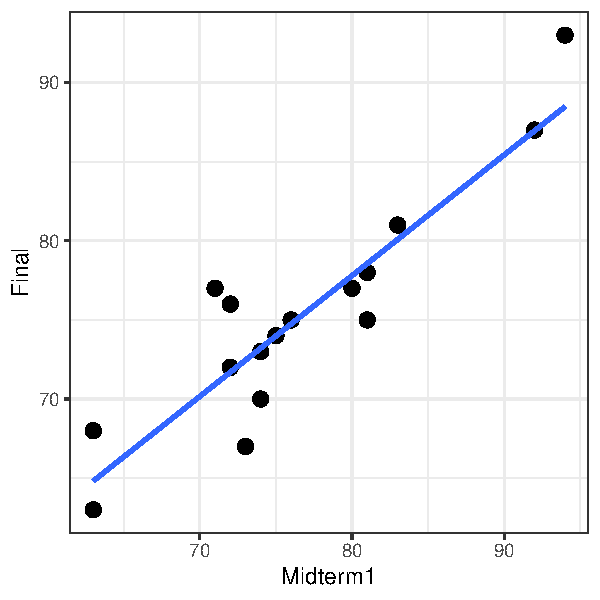
\includegraphics[scale=0.3]{figure-latex/unnamed-chunk-4-2-1}

  \textbf{Positive Relation}

  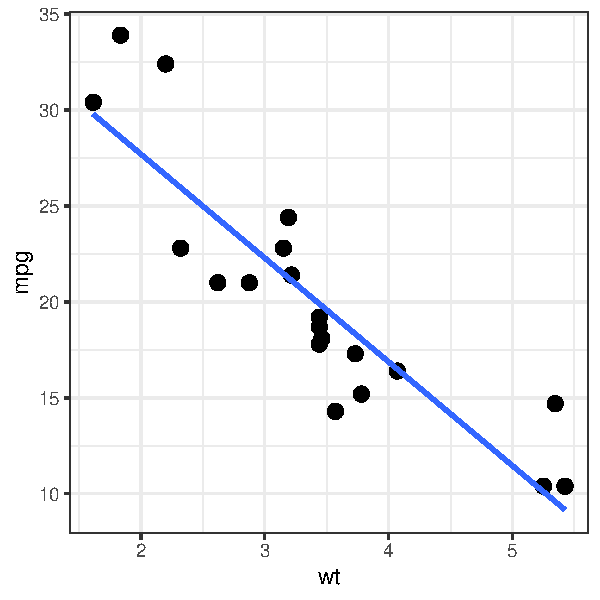
\includegraphics[scale=0.3]{figure-latex/unnamed-chunk-4-3-1}

  \textbf{Negative Relation}
  }

\begin{itemize}
  \item \textbf{Forms of relationship:}
\end{itemize}
\begin{minipage}{1.2\textwidth}
    \begin{minipage}[t]{0.3\textwidth}
      \begin{figure}[H]
        \begin{center}
          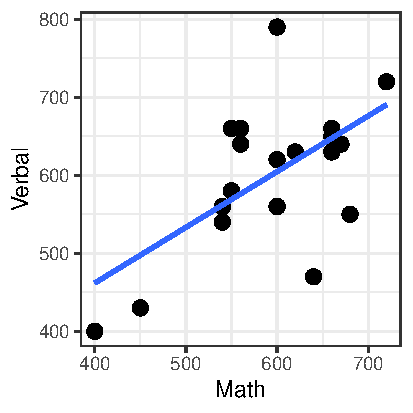
\includegraphics[scale=0.4]{figure-latex/unnamed-chunk-4-4-1}
          
          \textbf{Linear form}
        \end{center}
      \end{figure}
    \end{minipage}
    \begin{minipage}[t]{0.3\textwidth}
      \begin{figure}[H]
        \begin{center}
          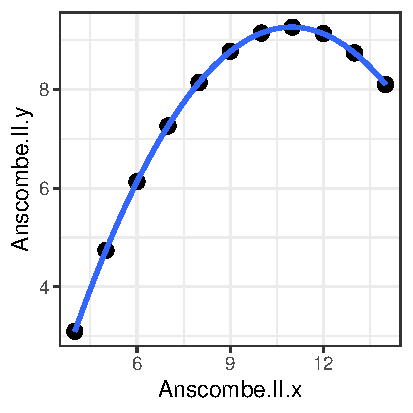
\includegraphics[scale=0.4]{figure-latex/unnamed-chunk-4-5-1}
          
          \textbf{Curvilinear form}
        \end{center}
      \end{figure}
    \end{minipage}
    \begin{minipage}[t]{0.3\textwidth}
      \begin{figure}[H]
        \begin{center}
          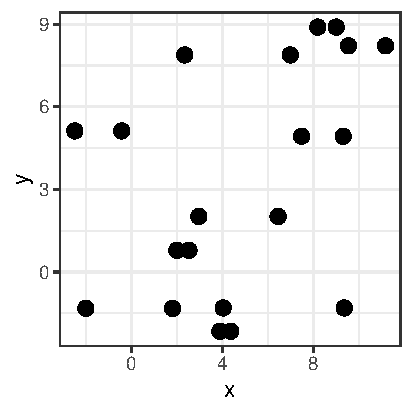
\includegraphics[scale=0.4]{figure-latex/unnamed-chunk-4-6-1}
          
          \textbf{No obvious relationship}
        \end{center}
      \end{figure}
    \end{minipage}
\end{minipage}

\begin{itemize}
\item
  The strength of the relationship is a description of how closely the
  data follow the form of the relationship.

  \begin{center}
    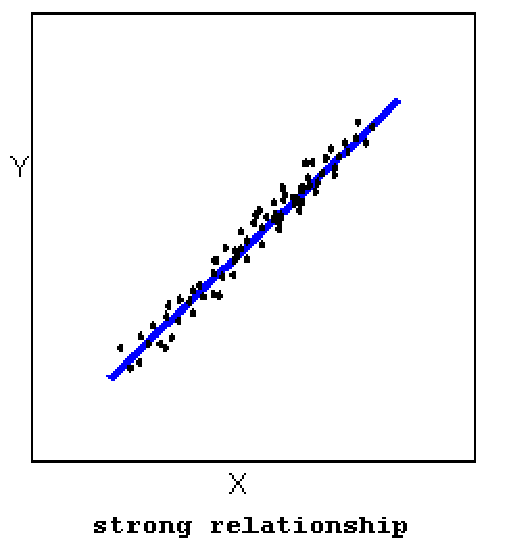
\includegraphics[scale=0.4]{Figures/strong-relation}
    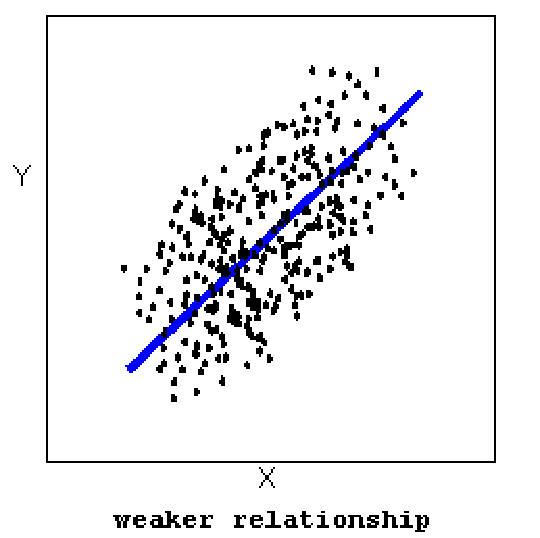
\includegraphics[scale=0.4]{Figures/weaker-relationship}
  \end{center}
\item
  Outliers are points that deviate from the pattern of the relationship.
\begin{center}
  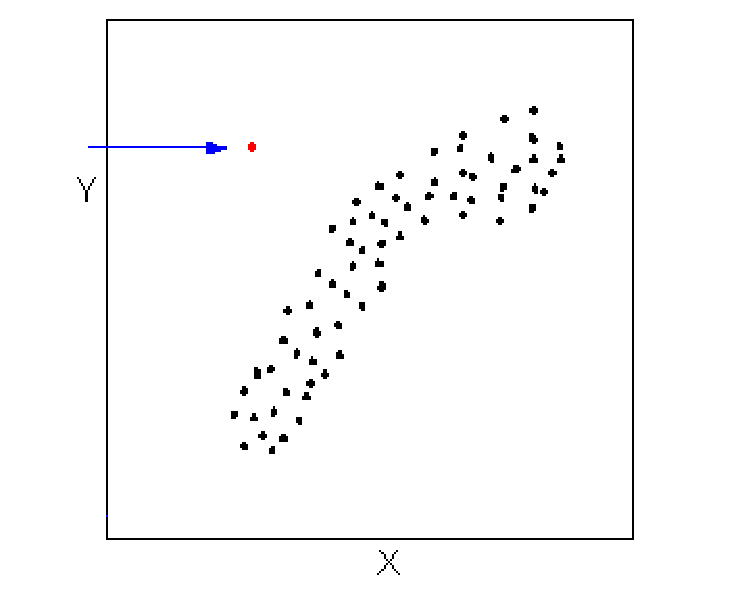
\includegraphics[scale=0.4]{Figures/outlier-in-relationship}
\end{center}
\end{itemize}

\begin{exercise}
Match scatterplots with the descriptions of relations between given variables.

\begin{center}
  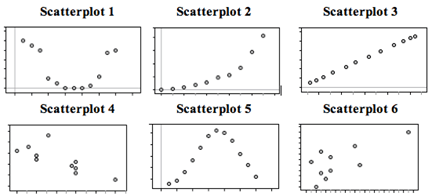
\includegraphics[width=0.8\textwidth]{Figures/MatchScatterplots.png}
\end{center}

\begin{enumerate}[sepno, label={\textbf{\Alph* :}}]
\item X = month (January = 1), Y = rainfall (inches) in Napa, CA
in 2010 (Note: Napa has rain in the winter months and months with little
to no rainfall in summer.)

\item X = month (January = 1), Y = average temperature in Boston
MA in 2010 (Note: Boston has cold winters and hot summers.)

\item X = year (in five-year increments from 1970),
Y = Medicare costs (in \$) (Note: the yearly increase in Medicare costs
has gotten bigger and bigger over time.)

\item X = average temperature in Boston MA (°F), Y = average
temperature in Boston MA (°C) each month in 2010

\item X = chest girth (cm), Y = shoulder girth (cm) for a sample
of men

\item X = engine displacement (liters), Y = city miles per gallon
for a sample of cars (Note: engine displacement is roughly a measure of
engine size. Large engines use more gas.)
\end{enumerate}

\end{exercise}

\hypertarget{the-correlation-coefficient}{%
\subsection{The Correlation
Coefficient}\label{the-correlation-coefficient}}

\begin{itemize}
\item
  The correlation coefficient \(r\) is a numeric measure that measures
  the strength and direction of a linear relationship between two
  quantitative variables. \[
  r=\dfrac{\sum\left(\frac{x-\bar{x}}{s_x}\right)\left(\frac{y-\bar{y}}{s_y}\right)}{n-1},
  \] where \(n\) is the sample size, \(x\) is a data value for the
  explanatory variable, \(\bar{x}\) is the mean of the \(x\)-values,
  \(s_x\) is the standard deviation of the \(x\)-values, and similarly,
  for the notations involving $y$.
\item
  The expression \(z=\frac{x-\bar{x}}{s_x}\) is known as the
  standardized variable (or \(z\)-score) which

  \begin{itemize}
  \item
    doesn't depend on the unit of the variable \(x\),
  \item
    has mean \(0\) and standard deviation 1.
  \end{itemize}
\item
  In Excel, the correlation coefficient can be calculated using the
  function \textsf{CORREL()}.
% \item
%   \href{https://courses.lumenlearning.com/wmopen-concepts-statistics/chapter/linear-relationships-2-of-4/}{Scatterplots
%   with different correlation coefficients}
\item
  \textbf{Rounding Rule:} Round to the nearest thousandth for \(r\),
  \(m\) and \(b\).
\item
  Geometric explanation of the definition of \(r\).
\end{itemize}

\begin{fullwidth}
  \colorbox{white}{
    \parbox{\linewidth}{
  \begin{multicols*}{2}
    \begin{center}
      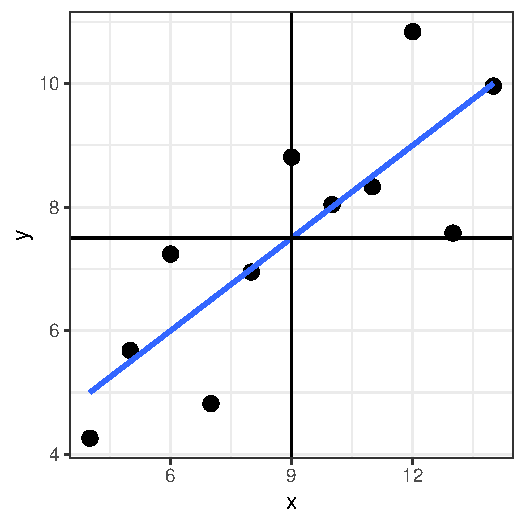
\includegraphics[width=0.6\linewidth]{figure-latex/unnamed-chunk-4-7-1}\\
      $r= 0.816$
    \end{center}

  \columnbreak

  \begin{center}
    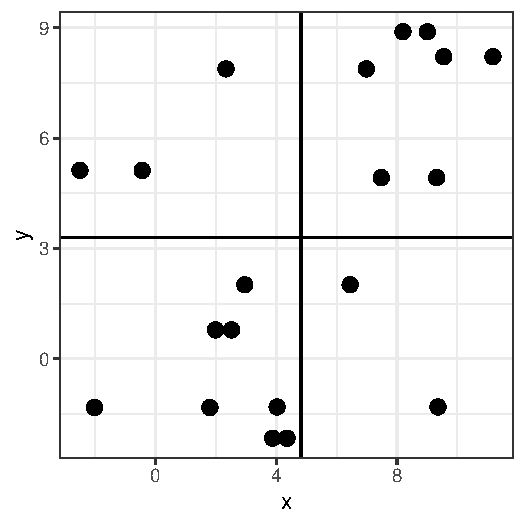
\includegraphics[width=0.6\linewidth]{figure-latex/unnamed-chunk-4-8-1}\\
    \(r=0.420\)
  \end{center}
\end{multicols*}
    }}
\end{fullwidth}


% \begin{remark}

% \begin{itemize}
% \item
%   \(r>0\) if all points \((x-\bar{x}, y-\bar{y})\) are in the 1st and
%   the 3rd quadrants.
% \item
%   \(r<0\) if all points \((x-\bar{x}, y-\bar{y})\) are in the 2nd and
%   the 4th quadrants.
% \end{itemize}

% \end{remark}

\begin{itemize}
\item
  The correlation coefficient \(r\) is between \(-1\) and \(1\).
\item
  The closer the absolute value \(|r|\) is to \(1\), the stronger the
  linear relationship is.
\item
  The correlation is symmetric in \(x\) and \(y\), that is
  \textsf{CORREL(x,\ y)=CORREL(y,\ x)}.
\item
  The correlation does not change when the units of measurement of
  either one of the variables change. In other words, if we change the
  units of measurement of the explanatory variable and/or the response
  variable, it has no effect on the correlation (r).
\item
  The correlation by itself is not enough to determine whether a
  relationship is linear. It's important to graph data set before
  analyzing it.\\
  \href{https://en.wikipedia.org/wiki/Anscombe\%27s_quartet}{https://en.wikipedia.org/wiki/Anscombe\%27s\_quartet}
\item
  The correlation is heavily influenced by outliers.
  \href{https://courses.lumenlearning.com/wmopen-concepts-statistics/chapter/linear-relationships-4-of-4/}{Try
  the simulation in Linear Relation (4 of 4) in Concepts in Statistics}
\item
  The reason that \(|r|\) is less than \(1\) is from the
  \href{https://en.wikipedia.org/wiki/Cauchy\%E2\%80\%93Schwarz_inequality}{Cauchy-Schwarz
  inequality}: \((\sum XY)^2\le \sum X^2\sum Y^2\).
\end{itemize}

\begin{exercise}

  Open the linked website and try  to guess the correlation coefficient.

\href{https://istats.shinyapps.io/guesscorr/}{https://istats.shinyapps.io/guesscorr/}

\end{exercise}

\begin{example}
  Use the data on Midterm 1 and Final from a sample of 10 students.
  \begin{itemize}
    \item
      Draw a scatter plot for the data table.
    \item
      Is it appropriate to study the relationship using a linear model.
    \item
      Find and interpret the correlation coefficient.
    \end{itemize}
  \begin{table}[h]
        \begin{tabular}[c]{l|l}
          \hline
          \multicolumn{1}{c|}{\textbf{Midterm1}} & 
          \multicolumn{1}{c}{\textbf{Final}} \\
          \hline
          72 & 72\\
          93 & 88\\
          81 & 82\\
          82 & 82\\
          94 & 88\\
          80 & 77\\
          73 & 78\\
          71 & 77\\
          81 & 76\\
          81 & 76\\
          63 & 68\\
          \hline
        \end{tabular}
  \end{table}
\end{example}
\vspace*{\baselineskip}

\begin{exercise}

Use the data shown below to answer the following questions.
\begin{itemize}
  \item
    Draw a scatter plot for the data table.
  \item
    Is it appropriate to study the relationship using a linear model.
  \item
    Find and interpret the correlation coefficient.
  \end{itemize}
  \begin{table}[h]
    \begin{small}
        \begin{tabular}[c]{l|l}
          \hline
          \multicolumn{1}{c|}{\textbf{$x$}} & 
          \multicolumn{1}{c}{\textbf{$y$}} \\
          \hline
          4 & 14.86 \\
          5 & 15.65 \\
          6 & 17.94 \\
          7 & 18.63 \\
          8 & 17.12 \\
          9 & 21.11 \\
          10 & 19.7 \\
          11 & 21.99 \\
          \hline
        \end{tabular}
    \end{small}
  \end{table}
\end{exercise}
\vspace*{2\baselineskip}

\hypertarget{correlation-v.s.-causation}{%
\subsection{Correlation v.s.
Causation}\label{correlation-v.s.-causation}}

\begin{itemize}
\item
  Correlation is described by data from observational study.
  Observational studies cannot prove cause and effect which requires
  controlled study and rigorous inferences.
\item
  Correlation may be used to make a prediction which is probabilistic.
\item
  In a linear relationship, an \(r\)-value that is close to 1 or -1 is
  insufficient to claim that the explanatory variable causes changes in
  the response variable. The correct interpretation is that there is a
  statistical relationship between the variables.
\item
  A \textbf{lurking variable} is a variable that is not measured in the
  study, but affects the interpretation of the relationship between the
  explanatory and response variables.
\end{itemize}

\begin{example}

The scatterplot below shows the relationship between the number of
firefighters sent to fires (x) and the amount of damage caused by fires
(y) in a certain city.
\begin{center}
  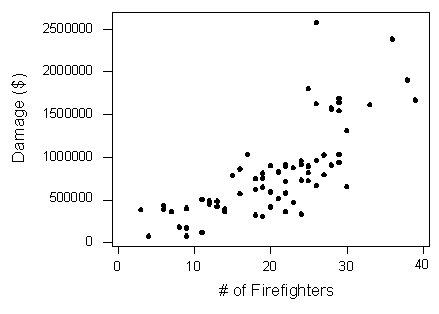
\includegraphics[scale=0.6]{Figures/scatterplot-firefigters.png}
\end{center}

Can we conclude that the increase in firefighters causes the increase in
damage?

\end{example}

\vspace*{2\baselineskip}

\begin{exercise}

Over a period of a few years, the population of Denver increased. It was
observed that during this period the correlation between the number of
people attending church and the number of people receiving traffic
tickets was \(r = 0.92\). Does going to church cause people to get
traffic tickets? Is there a lurking variable that might cause both
variables to increase?

\end{exercise}
\vspace*{2\baselineskip}

\hypertarget{the-regression-line}{%
\subsection{The Regression Line}\label{the-regression-line}}

\begin{itemize}
\item
  The line that best summarizes a linear relationship is \textbf{the
  least squares regression line}. The regression line is the line with
  the smallest sum of squares of the errors (\textbf{SSE}).
\item
  We use the least-squares regression line to predict the value
  \(\hat{y}\) for a value of the explanatory variable \(x\).
\item
  The regression line is unique and passes though
  \((\bar{x}, \bar{y})\). The equation is given by
  \[\hat{y}=m(x-\bar{x})+\bar{y}=m x+b,\] where the slope is
  \[m=\frac{\sum(x-\bar{x})(y-\bar{y})}{\sum(x-\bar{x})^2}=r\frac{s_y}{s_x}\]
  and the \(y\)-intercept is \(b=\bar{y}-m\bar{x}.\)
\item
  The \textbf{error of a prediction} is
  \[\text{Error}=\text{Observed}-\text{Predicted}=y-\hat{y}.\]
\item
  A prediction beyond the range of the data is called
  \textbf{extrapolation}.
\end{itemize}

\begin{example}
  The following sample is taken from data about the Old Faithful geyser.

  \begin{enumerate}[sepno]
    \item
      Study the linear relationship. Is it positive? What's the strength? What's the direction?
    \item
      Find the regression line, and the predicated value and the error if
      the eruption time is 1.8 minutes.
    \end{enumerate}

    \begin{tabular}[c]{l|l}
      \hline
      \multicolumn{1}{c|}{\textbf{eruptions}} & 
      \multicolumn{1}{c}{\textbf{waiting}} \\
      \hline
      3.917 & 84\\
      1.75 & 62\\
      4.200 & 78\\
      4.80 & 84\\
      1.750 & 47\\
      1.60 & 52\\
      4.700 & 83\\
      4.25 & 79\\
      2.167 & 52\\
      1.80 & 51\\
      \hline
    \end{tabular}
\end{example}

\vspace*{3\baselineskip}

\begin{exercise}
Research was conducted on the amount of training for 5K and the time a
contestant took to run the race. The researcher recorded the number of
miles during training ( a 1-month period) and the time to complete the
5K. The results are below.

\begin{longtable}[]{@{}ccccccc@{}}
\toprule()
Miles Trained & 20 & 69 & 102 & 29 & 46 & 68 \\
\midrule()
\endhead
Time(Minutes) & 37.26 & 38.3 & 39.96 & 29.95 & 26.56 & 43.78 \\
\bottomrule()
\end{longtable}
\begin{enumerate}
\item
  Find the correlation coefficient.
\item
  Find the equation of regression line.
\item
  Predict the time in the 5K if someone trained 29 miles.
\item
  Find the residual (the prediction error) for 102 miles trained.
\end{enumerate}

\end{exercise}

\hypertarget{assessing-the-fit-of-a-regression-line}{%
\subsection{Assessing the Fit of a Regression
Line}\label{assessing-the-fit-of-a-regression-line}}

\begin{itemize}
\item
  The prediction error is also called a \textbf{residual}. Another way
  to express the previous equation for error is
  \[y=\hat{y}+\text{residual}.\]
\item
  \textbf{Residual plots} are used to determine if a linear model is
  appropriate.

  A random pattern (or no obvious pattern) indicates a good fit of a
  linear model.
  \href{https://courses.lumenlearning.com/wmopen-concepts-statistics/chapter/assessing-the-fit-of-a-line-2-of-4/}{See
  Assessing the Fit of a Line (2 of 4) in Concepts in Statistics for
  examples.}
\item
  A ``typical'' error used to measure the fit of the regression is the
  \textbf{residual standard errors} (or \textbf{standard error of the
  regression}), calculated by the Excel function \textsf{STEYX()}, is
  \[s_e=\sqrt{\dfrac{SSE}{n-2}},\] where \(SSE=\sum (y-\hat{y})^2\) is
  the sum of square errors.
\item
  The smaller \(s_e\) is, the more accurate the prediction is.
\item
  The fit of a regression line can also be measured by the proportion of
  the variation in the response variable that is explained by the
  least-squares regression line. This proportion is known as the
  \textbf{coefficient of determination}.

  \begin{itemize}
  \item
    The \textbf{total variance} is \(SSD=\sum(y-\bar{y})^2\)
  \item
    The \textbf{explained variance} is \(SSR=\sum(\hat{y}-\bar{y})^2\).
  \item
    The \textbf{coefficient of determination} is
    \[r^2=\dfrac{SSR}{SSD}=\dfrac{\sum(\hat{y}-\bar{y})^2}{\sum(y-\bar{y})^2}.\]
  \end{itemize}
\end{itemize}

\begin{remark}

\begin{itemize}
\item
  The \(r\) in the coefficient of determination is the correlation
  coefficient. Equivalently, \(r=\pm\sqrt{r^2}\).
\item
  The smaller the standard error, the larger the coefficient of
  determination: \[r^2=1-\dfrac{SSE}{SSD}=1-\dfrac{(n-2)s_e^2}{SSD}.\]
\item
  \(n-2\) is the degrees of freedom. We lose two degrees of freedom
  because we estimate the slope and the \(y\)-intercept.
\item
  In a linear regression model \(Y=\beta_0 + \beta_1 X +\epsilon\), even
  we have \(\beta_0\) and \(\beta_1\) from the population, we still need
  estimate the standard deviation of error.
\end{itemize}

\end{remark}

\begin{example}

Find the standard error and coefficient of determination for the data of midterm1 and final.

\begin{table}[h]
      \begin{tabular}[c]{l|*{10}{c}}
        \hline
        \textbf{Midterm1} & 72 & 93 & 81 & 82 & 94 & 80 & 73 & 71 & 81 & 81\\
        \hline
\textbf{Final} & 72 & 88 & 82 & 82 & 88 & 77 & 78 & 77 & 76 & 76\\
        \hline
      \end{tabular}
\end{table}
\end{example}
\vspace*{5\baselineskip}

\begin{exercise}
A researcher measures the wrist circumference and height of a random
sample of individuals. The data are displayed below.

\begin{fullwidth}
  \colorbox{white}{
    \parbox{\linewidth}{
  \begin{center}
    \begin{tabular}[c]{l|*{10}{p{0.055\linewidth}}}
      \hline
        \textbf{Wrist Size (in)} & 5.5 & 5.6 & 5.8 & 5.9 & 6.1 & 6.3 & 6.4 & 6.5 & 6.6 & 6.8\\ 
        \hline
        \textbf{Height (in)} & 60.4 & 59.7 & 66.3 & 63.5 & 60.4 & 66.9 & 65.6 & 70.9 & 59.7 & 64.9 \\
      \hline
    \end{tabular}
  \end{center}
    }}
\end{fullwidth}

\begin{enumerate}
\item
  Find the equation of the best-fit line~\(y=mx+b\).~
\item
  Find the correlation coefficient.
\item
  Predict the height of a person with a wrist circumference of 6 inches
  using the best-fit line.
\item
  Calculate the residual for the point (6.5,70.9).
\item
  When predicting heights, what is a ``typical'' error of this linear
  model?
\item
  What proportion of variability in heights can be explained by this
  linear model? (Write your answer in decimal.)
\item
  Find the correlation coefficient if the heights are measured in feet.
\end{enumerate}

\end{exercise}

\hypertarget{lab-4-linear-regressions}{%
\subsection{Lab 4: Linear Regressions}\label{lab-4-linear-regressions}}

\begin{itemize}
\item
  To create a scatter plot, first select the data sets, and then look
  for \textsf{Insert\ Scatter(X,\ Y)} in the menu
  \textsf{Insert} $\rightarrow$ \textsf{Charts}.
\item
  The correlation coefficient \(r\) can be calculated by the Excel
  function \textsf{correl()}.
\item
  The slope of a linear regression can be calculated by the Excel
  function \textsf{SLOPE()}.
\item
  The \(y\)-intercept of a linear regression can be calculated by the
  Excel function \textsf{INTERCEPT()}.
\item
  The coefficient of determination can be calculated by first finding
  \(r\), then applying the formula \textsf{r\^{}2}.
\item
  The standard error of the regression (residual standard error) can be
  calculated by the Excel function \textsf{STEYX()}.
\end{itemize}

\begin{exercise}
  A researcher measures the wrist circumference and height of a random sample of individuals. The data and the scatterplot are displayed below.

  \begin{fullwidth}
    \colorbox{white}{
    \parbox{\linewidth}{
    \begin{center}
      \begin{tabular}[c]{l|*{12}{p{0.0375\linewidth}}}
      \hline  
      \textbf{Wrist Size (in)} &	5.7 & 5.9 & 6 & 6.2 & 6.3 & 6.5 & 6.7 & 7.1 & 7.3 & 8 & 8.2 & 8.4\\
      \hline
      \textbf{Height (in)} & 62.8 & 68.3 & 68.7 & 59.1 & 61.2 & 67.6 & 69.7 & 70.6 & 75.2 & 80.8 & 78.2 & 80.9\\
      \hline
      \end{tabular}
    \end{center}
    }}
  \end{fullwidth}

\begin{enumerate}
  \item Create a scatterplot for the data.
  \item Find the equation of the best-fit line $y=mx+b$.
  \item Predict the height of a person with a wrist circumference of 6 inches using the best-fit line. 
  \item Calculate the residual for the point (5.9,68.3). 
  \item When predicting heights, what is a "typical" error of this linear model? 
 \item What proportion of variability in heights can be explained by this linear model?
  \item Find the correlation coefficient if the heights are measured in feet. 
\end{enumerate}
\end{exercise}